\documentclass[]{article}
\usepackage[english,ukrainian]{babel}
\usepackage{amsmath}
\usepackage{multicol}
\usepackage{graphicx}

\begin{document}
$\;$

$\;$

$\;$

$\;$

$\;$

$\;$

$\;$

$\;$

$\;$

$\;$

$\;$

$\;$

$\;$

$\;$

$\;$

$\;$
\begin{center}
    \begin{huge}
    Домашня контрольна робота\\
    з Методів математичної фізики\\ 
    студента групи ОФ-91\\
    Сухова Олександра Сергійовича\\
    Варіант 10\\
    \end{huge}
\end{center}

\newpage

\begin{center}
    \textbf{Задача 1}
\end{center}
Умова:
\begin{equation*}
    \begin{cases}
      U_{tt}=\Delta U = U_{xx}+U_{yy}\\
      U\rvert_{t=0} = x\cdot y\cdot(6-x)\cdot(3-y)\\
      U_t\rvert_{t=0} = 0\\
      U\rvert_{x=0}= U\rvert_{y=0}=U\rvert_{x=6}=U\rvert_{y=3}=0\\
    \end{cases}
\end{equation*}
Шукатимемо розв'язок у вигляді добутку:
\[U(x,y,t) = X(x)\cdot Y(y)\cdot T(t)\]
Тоді:
\[\frac{T_{tt}}{T}=\frac{Y_{yy}}{Y}+\frac{X_{xx}}{X}\]

Методом розділення змінних:

\[\frac{X_{xx}}{X}=-\alpha,\;\;\;\frac{Y_{yy}}{Y}=-\beta,\;\;\; \frac{T_{tt}}{T}=-\alpha-\beta\]

З межових умов:

\[U\rvert_{x=0}=X(0)\cdot Y(y) \cdot T(t) = 0 \rightarrow X(0)=0\]
\[U\rvert_{y=0}=X(x)\cdot Y(0) \cdot T(t) = 0 \rightarrow Y(0)=0\]
\[U\rvert_{x=6}=X(6)\cdot Y(y) \cdot T(t) = 0 \rightarrow X(6)=0\]
\[U\rvert_{y=3}=X(x)\cdot Y(3) \cdot T(t) = 0 \rightarrow Y(3)=0\]

Маємо 2 однакові задачі Штурма Ліувілля:
\begin{multicols}{2}

    \begin{equation*}
        \begin{cases}
        X_{xx}+\alpha X = 0\\
        X(0)=0\\
        X(6)=0\\
        \end{cases}
    \end{equation*}

    \begin{equation*}
        \begin{cases}
        Y_{yy}+\beta Y = 0\\
        Y(0)=0\\
        Y(3)=0\\
        \end{cases}
    \end{equation*}
\end{multicols}

Їх розв'язки наступні:

\[X_n = sin\left(\frac{\pi n x}{6}\right),\;\;\alpha_n^2 = \left(\frac{\pi n}{6}\right)^2,\;\;n=1,2,\;...\]
\[Y_m = sin\left(\frac{\pi m x}{3}\right),\;\;\beta_m^2 = \left(\frac{\pi m}{3}\right)^2,\;\;m=1,2,\;...\]

Тоді:

\[T_{tt} = -\mu_{nm}^2\cdot T, \;\; \mu_{nm}^2=\left(\frac{\pi n}{6}\right)^2+\left(\frac{\pi m}{3}\right)^2\]

Маємо:
\[T_{nm}(t)=A_{nm}\cdot sin(\mu_{nm}\cdot t) + B_{nm}\cdot cos (\mu_{nm}\cdot t)\]

\[U(x,y,t) = \sum_{n=1}^{\infty}\sum_{m=1}^{\infty}T_{nm}(t)\cdot X_n(x)\cdot Y_m(y)\]

\newpage

Знайдемо $A_{nm}$ та $B_{nm}$ з початкових умов:
\[U_t(x,y,0) = 0 = \sum_{n=1}^{\infty}\sum_{m=1}^{\infty}\mu_{nm}\cdot A_{nm}\cdot X_n(x)\cdot Y_m(y)\rightarrow\;A_{nm} = 0, \;\forall n,m = 1,2,\;...\]
\[\left(A_{nm} = \frac{1}{\mu_{nm}}\cdot\frac{2}{6}\cdot\frac{2}{3}\int_{0}^{6}\int_{0}^{3}0\cdot sin\left(\frac{\pi n x}{6}\right)\cdot sin\left(\frac{\pi m y}{3}\right) dxdy = 0\right)\]

Оскільки:
\[U(x,y,0) = x\cdot y\cdot (6-x)\cdot (3-y) = \sum_{n=1}^{\infty}\sum_{m=1}^{\infty}B_{nm}\cdot X_n(x)\cdot Y_m(y)\]

\[B_{nm} = \frac{2}{6}\cdot\frac{2}{3}\int_{0}^{6}\int_{0}^{3}x\cdot y\cdot (6-x)\cdot (3-y)\cdot sin\left(\frac{\pi n x}{6}\right)\cdot sin\left(\frac{\pi m y}{3}\right) dxdy\]
Розглянемо інтеграл:
\begin{equation}
    I(a,l) = \frac{2}{a}\int_{0}^{a}z\cdot(a-z)\cdot sin\left(\frac{\pi l x}{a}\right)dz    
    \label{eq::1}
\end{equation}
Тоді:
\[B_{nm} = I(6,n)\cdot I(3,m)\]
Знайдемо \ref{eq::1} проінтегрувавши частинами:

\[I(a,l) = \frac{2}{a}\cdot \frac{a\cdot\left(\left(-2a^2-\pi^2al^2z+\pi^2l^2z^2\right)cos\left(\frac{\pi l z}{a}\right)+\pi a l\cdot(a-2z)sin\left(\frac{\pi l z}{a}\right)\right)}{\pi^3\cdot l^3}\bigg|_{0}^{a} = \]
\[=\frac{4\cdot a^2\left(1-(-1)^l\right)}{\pi^3\cdot l^3}\]
Маємо:
\[B_{nm} = \frac{144\cdot\left(1-(-1)^n\right)}{\pi^3\cdot n^3}\cdot\frac{36\cdot\left(1-(-1)^m\right)}{\pi^3\cdot m^3} = \frac{5184\cdot\left(1-(-1)^n\right)\cdot\left(1-(-1)^m\right)}{\pi^6\cdot n^3\cdot m^3}\]
\textbf{Відповідь:}
\[U(x,y,t) = \sum_{n=1}^{\infty}\sum_{m=1}^{\infty}\frac{5184\cdot\left(1-(-1)^n\right)\cdot\left(1-(-1)^m\right)}{\pi^6\cdot n^3\cdot m^3}sin\left(\frac{\pi n x}{6}\right)sin\left(\frac{\pi m y}{3}\right)\cdot\]\
\[\cdot cos\left(\pi\cdot t\sqrt{\left(\frac{n}{6}\right)^2+\left(\frac{m}{3}\right)^2}\right)\]

\newpage
\begin{center}
    \textbf{Задача 2}
\end{center}
Умова:
\begin{equation*}
    \begin{cases}
      U_{tt}=10\Delta U = 10\left(\frac{\partial^2}{\partial r^2}+\frac{1}{r}\frac{\partial}{\partial r}\right)U\\
      0\leq r<16\\
      0<t<\infty\\
      U(16,t) = 0\\
      U(r,0) = \frac{1}{8}\left(1-\left(\frac{r}{16}\right)^2\right)\\
      U_t(r,0) = 0\\
    \end{cases}
\end{equation*}
Шукатимемо розв'язок у вигляді добутку:
\[U(r,t) = R(r)\cdot T(t)\]
З межової умови:
\[U(16,t)=0=R(16)\cdot T(t)\rightarrow R(16)=0\]
Методом розділення змінних:
\[\frac{T_{tt}}{10T}=\left(\frac{R''+\frac{1}{r}R'}{R}\right)=-\lambda\]
Маємо рівняння:
\[r^2R''+rR'+\lambda r^2R=0\]
Зробимо заміну $\sqrt{\lambda} r = \rho$, маємо рівняння Бесселя 0-го порядку:
\[\rho^2R''+\rho R'+\left(\rho^2-0^2\right)R=0\]
Розв'язком якого є:
\[R = A\cdot J_0(\rho)+B\cdot N_0(\rho) = A\cdot J_0(\sqrt{\lambda}r)+B\cdot N_0(\sqrt{\lambda}r) \]
Оскільки $\big|U(r,t)\big|<\infty\rightarrow\big|R(r)\big|<\infty,\;\;\forall r: 0\leq r<16$:
\[B = 0\;\left(\lim_{r\rightarrow +0} N_0(r) = -\infty\right)\]
З межової умови:
\[R(16) = A\cdot J_0(\sqrt{\lambda}\cdot 16) = 0 \rightarrow \sqrt{\lambda_n} = \frac{\chi_n}{16}, n = 1,2,\;...\]
\newpage
Нулі функції Бесселя 0-го порядку$\left(\chi_n\right)$ показані на рисунку нижче:
\begin{figure}[!h]
    \center{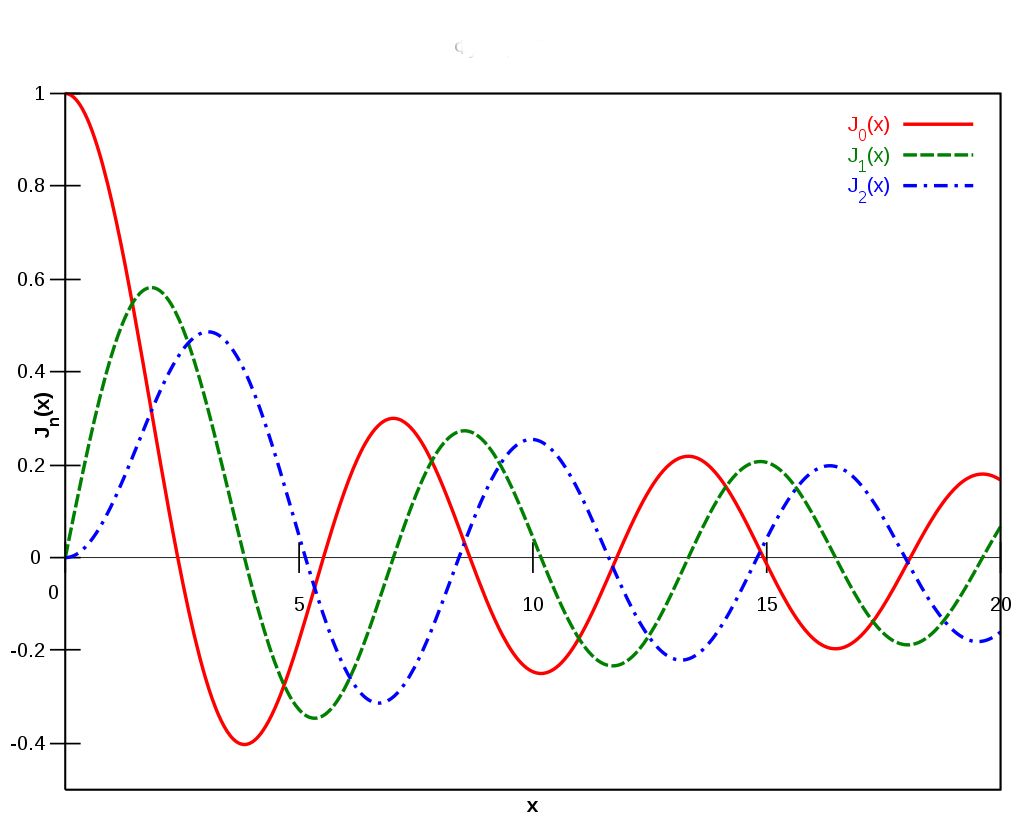
\includegraphics[width=0.8\linewidth, height=7.5cm]{1.png}}
    \label{fig:flow}
\end{figure}

Тоді:

\[T_{tt} = -10\left(\frac{\chi_n}{16}\right)^2T\]
\[T_n = A_n\cdot sin\left(\frac{\sqrt{10}\chi_n t}{16}\right)+ B_n cos\left(\frac{\sqrt{10}\chi_n t}{16}\right)\]

Маємо:
\[U(r,t) = \sum_{n=1}^{\infty}\left(A_n\cdot sin\left(\frac{\sqrt{10}\chi_n t}{16}\right)+ B_n cos\left(\frac{\sqrt{10}\chi_n t}{16}\right)\right) J_0\left(\frac{\chi_n r}{16}\right)\]

Знайдемо $A_n$ та $B_n$ з початкових умов:

\[U_t(r,0) = \sum_{n=1}^{\infty}\left(\frac{\sqrt{10}\chi_n}{16}\cdot A_n\right) J_0\left(\frac{\chi_n r}{16}\right) = 0\rightarrow\;A_{n} = 0, \;\forall n = 1,2,\;...\]
\[\left(A_n = \frac{2}{16\cdot \chi_n\cdot\sqrt{10}\left(J_0^{'}(\chi_n)\right)^2}\int_{0}^{16}r\cdot 0\cdot J_0\left(\frac{\chi_n r}{16}\right)dr = 0\right)\]

Оскільки:
\[U(r,0) = \sum_{n=1}^{\infty}B_n\cdot J_0\left(\frac{\chi_n r}{16}\right) = \frac{1}{8}\left(1-\left(\frac{r}{16}\right)^2\right)\]

\newpage

Маємо:

\[B_n = \frac{2}{256\left(J_0^{'}(\chi_n)\right)^2}\int_{0}^{16}r\cdot \frac{1}{8}\left(1-\left(\frac{r}{16}\right)^2\right)\cdot J_0\left(\frac{\chi_n r}{16}\right)dr\]

Використаємо наступні властивості інтегралів з функціями Бесселя:

\[\int x\cdot J_0(x) dx = x\cdot J_1(x) + C\]

\[\int x\cdot J_0(x)\cdot x^2 dx = x^3\cdot J_1(x) - 2\cdot x^2 J_2(x)+ C\]

Маємо:

\[B_n = \frac{1}{4\cdot\chi_n\left(J_0^{'}(\chi_n)\right)^2}\cdot\int_{0}^{\chi_n} \frac{z}{\chi_n}\cdot\left(1-\left(\frac{z}{\chi_n}\right)^2\right)\cdot J_0\left(z\right) = \]
\[ = \frac{1}{4\cdot\chi_n\left(J_0^{'}(\chi_n)\right)^2} \cdot \left(\frac{z}{\chi_n}\cdot J_1(z)-\frac{1}{\chi_n^3}\cdot\left(z^3\cdot J_1(z)-2\cdot z^2\cdot J_2(z)\right)\right)\big|_0^{\chi_n} = \]
\[ = \frac{1}{4\cdot\chi_n\left(J_0^{'}(\chi_n)\right)^2} \cdot \left( J_1(\chi_n) - J_1(\chi_n)+\frac{2}{\chi_n}\cdot J_2 (\chi_n)\right) = \]
\[ = \big| J_{\nu-1}(x)+J_{\nu+1}(x) = \frac{2\cdot\nu}{x}J_\nu(x),\;\;\nu=2 \big| =\]
\[= \frac{1}{4\cdot\chi_n\left(J_0^{'}(\chi_n)\right)^2}\left(J_1(\chi_n)-\frac{2}{\chi_n}J_2(\chi_n)+J_3(\chi_n)\right)\]

\textbf{Відповідь:}

\[U(r,t) = \sum_{n=1}^{\infty} \frac{1}{4\cdot\chi_n\left(J_0^{'}(\chi_n)\right)^2}\left(J_1(\chi_n)-\frac{2}{\chi_n}J_2(\chi_n)+J_3(\chi_n)\right)\cdot cos\left(\frac{\sqrt{10}\chi_n t}{16}\right)\cdot J_0\left(\frac{\chi_n r}{16}\right)\]

\newpage
\begin{center}
    \textbf{Задача 3}
\end{center}
Умова:
\begin{equation*}
    \begin{cases}
      U_{t}=\Delta U  = \left(\frac{\partial^2}{\partial r^2}+\frac{1}{r}\frac{\partial}{\partial r}\right)U\\
      0\leq r<5\\
      0<t<\infty\\
      U(r,0) = 25-r^2\\
      U(5,t) = 0\\
    \end{cases}
\end{equation*}
Шукатимемо розв'язок у вигляді добутку:

\[U(r,t) = R(r)\cdot T(t)\]
З межової умови:
\[U(5,t)=0=R(5)\cdot T(t)\rightarrow R(5)=0\]
Методом розділення змінних:
\[\frac{T_{t}}{T}=\left(\frac{R''+\frac{1}{r}R'}{R}\right)=-\lambda\]
Маємо рівняння:
\[r^2R''+rR'+\lambda r^2R=0\]
Зробимо заміну $\sqrt{\lambda} r = \rho$, маємо рівняння Бесселя 0-го порядку:
\[\rho^2R''+\rho R'+\left(\rho^2-0^2\right)R=0\]
Розв'язком якого є:
\[R = A\cdot J_0(\rho)+B\cdot N_0(\rho) = A\cdot J_0(\sqrt{\lambda}r)+B\cdot N_0(\sqrt{\lambda}r) \]
Оскільки $\big|U(r,t)\big|<\infty\rightarrow\big|R(r)\big|<\infty,\;\;\forall r: 0\leq r<5$:
\[B = 0\;\left(\lim_{r\rightarrow +0} N_0(r) = -\infty\right)\]
З межової умови:
\[R(5) = A\cdot J_0(\sqrt{\lambda}\cdot 5) = 0 \rightarrow \sqrt{\lambda_n} = \frac{\chi_n}{5}, n = 1,2,\;...\]
\newpage
Нулі функції Бесселя 0-го порядку$\left(\chi_n\right)$ показані на рисунку нижче:
\begin{figure}[!h]
    \center{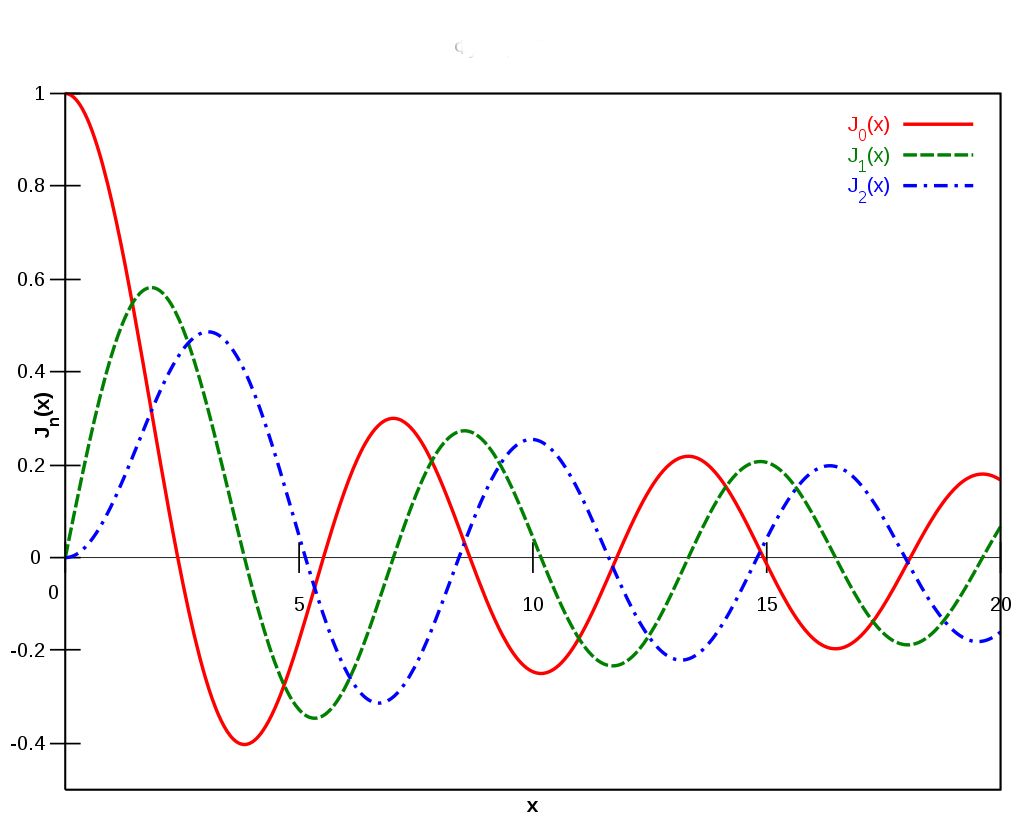
\includegraphics[width=0.8\linewidth, height=7.5cm]{1.png}}
    \label{fig:flow}
\end{figure}

Тоді:

\[T_{t} = -\left(\frac{\chi_n}{5}\right)^2T\]
\[T_n = A_n\cdot e^{-\left(\frac{\chi_n}{5}\right)^2\cdot t}\]

Маємо:
\[U(r,t) = \sum_{n=1}^{\infty}A_n\cdot e^{-\left(\frac{\chi_n}{5}\right)^2\cdot t}J_0\left(\frac{\chi_n r}{5}\right)\]

Знайдемо $A_n$ початкової умови:

\[U(r,0) = \sum_{n=1}^{\infty}A_n\cdot J_0\left(\frac{\chi_n r}{5}\right) = 25 - r^2\]

Маємо:

\[A_n = \frac{2}{25\left(J_0^{'}(\chi_n)\right)^2}\int_{0}^{5}r\cdot \left(25-r^2\right)\cdot J_0\left(\frac{\chi_n r}{5}\right)dr\]

Використаємо наступні властивості інтегралів з функціями Бесселя:

\[\int x\cdot J_0(x) dx = x\cdot J_1(x) + C\]

\[\int x\cdot J_0(x)\cdot x^2 dx = x^3\cdot J_1(x) - 2\cdot x^2 J_2(x)+ C\]

Маємо:

\[A_n = \frac{2}{25\left(J_0^{'}(\chi_n)\right)^2}\cdot\int_{0}^{\chi_n} \frac{z}{\chi_n}\cdot\left(1-\left(\frac{z}{\chi_n}\right)^2\right)\cdot J_0\left(z\right) = \]
\[ = \frac{2}{25\left(J_0^{'}(\chi_n)\right)^2} \cdot \left(\frac{z}{\chi_n}\cdot J_1(z)-\frac{1}{\chi_n^3}\cdot\left(z^3\cdot J_1(z)-2\cdot z^2\cdot J_2(z)\right)\right)\big|_0^{\chi_n} = \]
\[ = \frac{2}{25\left(J_0^{'}(\chi_n)\right)^2} \cdot \left( J_1(\chi_n) - J_1(\chi_n)+\frac{2}{\chi_n}\cdot J_2 (\chi_n)\right) = \]
\[ = \big| J_{\nu-1}(x)+J_{\nu+1}(x) = \frac{2\cdot\nu}{x}J_\nu(x),\;\;\nu=2 \big| = \]
\[= \frac{2}{25\left(J_0^{'}(\chi_n)\right)^2}\left(J_1(\chi_n)-\frac{2}{\chi_n}J_2(\chi_n)+J_3(\chi_n)\right)\]

\textbf{Відповідь:}

\[U(r,t) = \sum_{n=1}^{\infty} \frac{2}{25\left(J_0^{'}(\chi_n)\right)^2}\left(J_1(\chi_n)-\frac{2}{\chi_n}J_2(\chi_n)+J_3(\chi_n)\right)\cdot e^{-\left(\frac{\chi_n}{5}\right)^2\cdot t}\cdot J_0\left(\frac{\chi_n r}{5}\right)\]






\end{document}